\documentclass[a4paper,11pt,fleqn,dvipsnames,twoside,openany]{memoir} 	% Openright aabner kapitler paa hoejresider (openany begge)

%%%% PACKAGES %%%%

% ¤¤ Oversaettelse og tegnsaetning ¤¤ %
\usepackage[utf8]{inputenc}					% Input-indkodning af tegnsaet (UTF8)
\usepackage[english]{babel}					% Dokumentets sprog
\usepackage[T1]{fontenc}					% Output-indkodning af tegnsaet (T1)
\usepackage{ragged2e,anyfontsize}			% Justering af elementer
\usepackage{fixltx2e}						% Retter forskellige fejl i LaTeX-kernen
																			
% ¤¤ Figurer og tabeller (floats) ¤¤ %
\usepackage{graphicx} 						% Haandtering af eksterne billeder (JPG, PNG, EPS, PDF)
%\usepackage{eso-pic}						% Tilfoej billedekommandoer paa hver side
%\usepackage{wrapfig}						% Indsaettelse af figurer omsvoebt af tekst. \begin{wrapfigure}{Placering}{Stoerrelse}
\usepackage{multirow}                		% Fletning af raekker og kolonner (\multicolumn og \multirow)
\usepackage{multicol}         	        	% Muliggoer output i spalter
\usepackage{rotating}						% Rotation af tekst med \begin{sideways}...\end{sideways}
\usepackage{colortbl} 						% Farver i tabeller (fx \columncolor og \rowcolor)
\usepackage[table]{xcolor}				 	% Definer farver med \definecolor. Se mere: http://en.wikibooks.org/wiki/LaTeX/Colors
\usepackage{flafter}						% Soerger for at floats ikke optraeder i teksten foer deres reference
\let\newfloat\relax 						% Justering mellem float-pakken og memoir
\usepackage{float}							% Muliggoer eksakt placering af floats, f.eks. \begin{figure}[H]
\usepackage{wrapfig}



% ¤¤ Matematik mm. ¤¤
\usepackage{amsmath,amssymb,stmaryrd} 		% Avancerede matematik-udvidelser
\usepackage{mathtools}						% Andre matematik- og tegnudvidelser
\usepackage{textcomp}                 		% Symbol-udvidelser (f.eks. promille-tegn med \textperthousand )
\usepackage{rsphrase}						% Kemi-pakke til RS-saetninger, f.eks. \rsphrase{R1}
\usepackage[version=3]{mhchem} 				% Kemi-pakke til flot og let notation af formler, f.eks. \ce{Fe2O3}
\usepackage{siunitx}						% Flot og konsistent praesentation af tal og enheder med \si{enhed} og \SI{tal}{enhed}
\sisetup{locale=DE}							% Opsaetning af \SI (DE for komma som decimalseparator) 

% ¤¤ Referencer og kilder ¤¤ %
\usepackage[danish]{varioref}				% Muliggoer bl.a. krydshenvisninger med sidetal (\vref)
\usepackage[square,sort,comma,numbers]{natbib}							% Udvidelse med naturvidenskabelige citationsmodeller
%\usepackage{xr}							% Referencer til eksternt dokument med \externaldocument{<NAVN>}
%\usepackage{glossaries}					% Terminologi- eller symbolliste (se mere i Daleifs Latex-bog)

% ¤¤ Misc. ¤¤ %
\usepackage{lipsum}							% Dummy text \lipsum[..]
\usepackage[shortlabels]{enumitem}			% Muliggoer enkelt konfiguration af lister
\usepackage{pdfpages}						% Goer det muligt at inkludere pdf-dokumenter med kommandoen \includepdf[pages={x-y}]{fil.pdf}	
\pdfoptionpdfminorversion=6					% Muliggoer inkludering af pdf dokumenter, af version 1.6 og hoejere
\pretolerance=2500 							% Justering af afstand mellem ord (hoejt tal, mindre orddeling og mere luft mellem ord)

% Kommentarer og rettelser med \fxnote. Med 'final' i stedet for 'draft' udloeser hver note en error i den faerdige rapport.
\usepackage[footnote,final,english,silent,nomargin]{fixme}		
\usepackage[bottom]{footmisc}

%%%% CUSTOM SETTINGS %%%%

% ¤¤ Marginer ¤¤ %
\setlrmarginsandblock{3.5cm}{2.5cm}{*}		% \setlrmarginsandblock{Indbinding}{Kant}{Ratio}
\setulmarginsandblock{2.5cm}{3.0cm}{*}		% \setulmarginsandblock{Top}{Bund}{Ratio}
\checkandfixthelayout 						% Oversaetter vaerdier til brug for andre pakker

%	¤¤ Afsnitsformatering ¤¤ %
\setlength{\parindent}{0mm}           		% Stoerrelse af indryk
\setlength{\parskip}{3mm}          			% Afstand mellem afsnit ved brug af double Enter
\linespread{1,1}							% Linie afstand

% ¤¤ Litteraturlisten ¤¤ %
%\bibpunct[,]{[}{]}{;}{a}{,}{,} 				% Definerer de 6 parametre ved Harvard henvisning (bl.a. parantestype og seperatortegn)
%\bibliographystyle{bibtex/harvard}			% Udseende af litteraturlisten.
\bibliographystyle{ieeetr}	

% ¤¤ Indholdsfortegnelse ¤¤ %
\setsecnumdepth{subsection}		 			% Dybden af nummerede overkrifter (part/chapter/section/subsection)
\maxsecnumdepth{subsection}					% Dokumentklassens graense for nummereringsdybde
\settocdepth{section} 					% Dybden af indholdsfortegnelsen

% ¤¤ Lister ¤¤ %
\setlist{
  topsep=0pt,								% Vertikal afstand mellem tekst og listen
  itemsep=-1ex,								% Vertikal afstand mellem items
} 

% ¤¤ Visuelle referencer ¤¤ %
\usepackage[colorlinks]{hyperref}			% Danner klikbare referencer (hyperlinks) i dokumentet.
\hypersetup{colorlinks = true,				% Opsaetning af farvede hyperlinks (interne links, citeringer og URL)
    linkcolor = black,
    citecolor = black,
    urlcolor = black
}

% ¤¤ Opsaetning af figur- og tabeltekst ¤¤ %
\captionnamefont{\small\bfseries\itshape}	% Opsaetning af tekstdelen ('Figur' eller 'Tabel')
\captiontitlefont{\small}					% Opsaetning af nummerering
\captiondelim{. }							% Seperator mellem nummerering og figurtekst
\hangcaption								% Venstrejusterer flere-liniers figurtekst under hinanden
\captionwidth{\linewidth}					% Bredden af figurteksten
\setlength{\belowcaptionskip}{10pt}			% Afstand under figurteksten
		
% ¤¤ Navngivning ¤¤ %
\addto\captionsdanish{
	\renewcommand\appendixname{Appendiks}
	\renewcommand\contentsname{Indholdsfortegnelse}	
	\renewcommand\appendixpagename{Appendiks}
	\renewcommand\appendixtocname{Appendiks}
	\renewcommand\cftchaptername{\chaptername~}				% Skriver "Kapitel" foran kapitlerne i indholdsfortegnelsen
	\renewcommand\cftappendixname{\appendixname~}			% Skriver "Appendiks" foran appendiks i indholdsfortegnelsen
}

% ¤¤ Kapiteludssende ¤¤ %
\definecolor{numbercolor}{gray}{0.7}		% Definerer en farve til brug til kapiteludseende
\newif\ifchapternonum

\makechapterstyle{E4}{					% Definerer kapiteludseende frem til ...
  \renewcommand\beforechapskip{0pt}
  \renewcommand\printchaptername{}
  \renewcommand\printchapternum{}
  \renewcommand\printchapternonum{\chapternonumtrue}
  \renewcommand\chaptitlefont{\fontfamily{pbk}\fontseries{db}\fontshape{n}\fontsize{25}{35}\selectfont\raggedleft}
  \renewcommand\chapnumfont{\fontfamily{pbk}\fontseries{m}\fontshape{n}\fontsize{1in}{0in}\selectfont\color{numbercolor}}
  \renewcommand\printchaptertitle[1]{%
    \noindent
    \ifchapternonum
    \begin{tabularx}{\textwidth}{X}
    {\let\\\newline\chaptitlefont ##1\par} 
    \end{tabularx}
    \par\vskip-2.5mm\hrule
    \else
    \begin{tabularx}{\textwidth}{Xl}
    {\parbox[b]{\linewidth}{\chaptitlefont ##1}} & \raisebox{-15pt}{\chapnumfont \thechapter}
    \end{tabularx}
    \par\vskip2mm\hrule
    \fi
  }
}											% ... her

\chapterstyle{E4}						% Valg af kapiteludseende - Google 'memoir chapter styles' for alternativer

% ¤¤ Sidehoved ¤¤ %

\makepagestyle{IHA}							% Definerer sidehoved og sidefod udseende frem til ...
\makepsmarks{IHA}{%
	\createmark{chapter}{left}{shownumber}{}{. \ }
	\createmark{section}{right}{shownumber}{}{. \ }
	\createplainmark{toc}{both}{\contentsname}
	\createplainmark{lof}{both}{\listfigurename}
	\createplainmark{lot}{both}{\listtablename}
	\createplainmark{bib}{both}{\bibname}
	\createplainmark{index}{both}{\indexname}
	\createplainmark{glossary}{both}{\glossaryname}
}
\nouppercaseheads											% Ingen Caps oenskes

\makeevenhead{IHA}{\leftmark}{}{Ingeniørhøjskolen i Aarhus}								% Definerer lige siders sidehoved (\makeevenhead{Navn}{Venstre}{Center}{Hoejre})
\makeoddhead{IHA}{\leftmark}{}{Ingeniørhøjskolen i Aarhus}		% Definerer ulige siders sidehoved (\makeoddhead{Navn}{Venstre}{Center}{Hoejre})
\makeevenfoot{IHA}{}{\thepage}{}								% Definerer lige siders sidefod (\makeevenfoot{Navn}{Venstre}{Center}{Hoejre})
\makeoddfoot{IHA}{}{\thepage}{}									% Definerer ulige siders sidefod (\makeoddfoot{Navn}{Venstre}{Center}{Hoejre})
\makeheadrule{IHA}{\textwidth}{0.5pt}							% Tilfoejer en streg under sidehovedets indhold
\makefootrule{IHA}{\textwidth}{0.5pt}{1mm}						% Tilfoejer en streg under sidefodens indhold

\copypagestyle{IHAchap}{IHA}								% Sidehoved for kapitelsider defineres som standardsider, men med blank sidehoved
\makeoddhead{IHAchap}{}{}{}
\makeevenhead{IHAchap}{}{}{}
\makeheadrule{IHAchap}{\textwidth}{0pt}
\makefootrule{IHAchap}{\textwidth}{0.5pt}{1mm}						% Tilfoejer en streg under sidefodens indhold
\aliaspagestyle{chapter}{IHAchap}							% Den ny style vaelges til at gaelde for chapters
															% ... her
															
\pagestyle{IHA}												% Valg af sidehoved og sidefod


%%%% CUSTOM COMMANDS %%%%

% ¤¤ Billede hack ¤¤ %
\newcommand{\figur}[4]{
		\begin{figure}[H] \centering
			\includegraphics[width=#1\textwidth]{billeder/#2}
			\caption{#3}\label{#4}
		\end{figure} 
}

% ¤¤ Tab hack ¤¤ %
\newcommand{\tab}[1]{\hspace{.2\textwidth}\rlap{#1}}

% ¤¤ Specielle tegn ¤¤ %
\newcommand{\grader}{^{\circ}\text{C}}
\newcommand{\gr}{^{\circ}}
\newcommand{\g}{\cdot}


%%%% ORDDELING %%%%

\hyphenation{}

%%%% FARVER %%%%
\definecolor{light-gray}{gray}{0.95}

\usepackage{listings}
\usepackage{color} %red, green, blue, yellow, cyan, magenta, black, white
\definecolor{mygreen}{RGB}{28,172,0} % color values Red, Green, Blue
\definecolor{mylilas}{RGB}{170,55,241}

\usepackage{algorithmicx}
\usepackage{algpseudocode}
\usepackage{algorithm}
\raggedbottom
\begin{document}

\lstset{language=Matlab,%
    %basicstyle=\color{red},
    breaklines=true,%
    morekeywords={matlab2tikz},
    keywordstyle=\color{blue},%
    morekeywords=[2]{1}, keywordstyle=[2]{\color{black}},
    identifierstyle=\color{black},%
    stringstyle=\color{mylilas},
    commentstyle=\color{mygreen},%
    showstringspaces=false,%without this there will be a symbol in the places where there is a space
    numbers=left,%
    numberstyle={\tiny \color{black}},% size of the numbers
    numbersep=9pt, % this defines how far the numbers are from the text
    emph=[1]{for,end,break},emphstyle=[1]\color{red}, %some words to emphasise
    %emph=[2]{word1,word2}, emphstyle=[2]{style},    
}

%\pagestyle{empty}
\newcommand{\HRule}{\rule{\linewidth}{0.5mm}} % Defines a new command for the horizontal lines, change thickness here

\begin{center} % Center everything on the page
 
%----------------------------------------------------------------------------------------
%	HEADING SECTIONS
%----------------------------------------------------------------------------------------

\textsc{\LARGE Engineering college of Aarhus}\\[1.5cm] % Name of your university/college
%\textsc{\large Spring 2014}\\[0.5cm] % Minor heading such as course title

%----------------------------------------------------------------------------------------
%	TITLE SECTION
%----------------------------------------------------------------------------------------

\HRule \\[0.4cm]
{ \Large \bfseries \textsc{HLS Reading Course report}}\\[0.4cm] % Bachelor project title
{ \huge \bfseries \textsc{XILINX HLS Directives, How and Why?}} % Document title
\HRule \\[1.5cm]

%----------------------------------------------------------------------------------------
%	AUTHOR SECTION
%----------------------------------------------------------------------------------------
\begin{center}
\begin{Large}\textit{Supervisor:}\end{Large}\\
\ \\
Kim Bjerge\\
kbe\begin{Large}@\end{Large}iha.dk
\end{center}
\ \\
\ \\
\begin{table}[H]
\centering
\begin{tabular}{p{4cm} c p{4cm}}
\multicolumn{3}{c}{\begin{Large}\textit{Author:}\end{Large}}\\
\\
\\
\cline{1-1} \cline{3-3}\\
Nicolai Glud &  \\
20093625 
\end{tabular}
\end{table}
\ \\

\vspace{5cm}


%----------------------------------------------------------------------------------------
\begin{figure}[H]
\centering

\includegraphics[scale=.5]{billeder/au-ingenioerhoejskolen_en}
\end{figure}

\vfill
\textsc{\large Department of electronic engineering}\\[0.5cm]
%----------------------------------------------------------------------------------------
%	DATE SECTION
%----------------------------------------------------------------------------------------

{\large \today}\\[3cm] % Date, change the \today to a set date if you want to be precise
\end{center}
 
\pagestyle{IHA}
\tableofcontents
\setcounter{page}{2}
\chapter{Introduction}
The goal of this report is research some of the uses for high level synthesis. An example problem from another course will be used as basis for the research and methods acquired in this course will be applied to the problem. A Comparison of the different methods will be presented with regards to relevant measurements.

A series of questions will be explored and answered in the case study. These questions are:
\begin{itemize}
\item What are optimisation directives in High-Level synthesis?
\item How are they used and to what effect?
\end{itemize}
To answer these questions a small subset of the optimisation directives are chosen and applied to the aforementioned example problem. 

The overall purpose of the report is described in the course catalogue as these points:
\begin{itemize}
\item Define and explain concepts, methods and technologies relating to the chosen subject area.
\item Give an account of research articles relevant to the subject area.
\item Account for the status and application of the subject area.
\item Prepare a report and an oral presentation on the subject area.
\end{itemize}
  
\chapter{Study}
Animals move around when searching for things like food or a mate. Some animals move in seemingly random patterns but the interesting question is: "Is there an underlying pattern or model that describes this behaviour".\\
When talking about animal movement behavioural animals might use a reaction-diffusion process. This process entails the movement (diffusion) and the interaction with the environment (reaction). Reaction is often described as finding food, mating a mate or finding a predator. All of these things force the animal into changing its movement behaviour. This could mean a stop in a long search for example. Reaction behaviour will not be a part of this report.

\section{Diffusion processes}
Diffusion processes can also be called walks. This section seeks to explain some of the different walks and what is characteristic about them.

\subsection{Brownian motion}
Brownian motion is a type of random walk where the motion follows a Gaussian distribution. In mathematically terms this can be shown as follows:
\begin{equation}
P($Step size$) \sim \mathcal{N}(0,t-s) ($for $ 0 \leq s \leq t)
\label{eq:brownianm}
\end{equation}
This type of diffusion where the variance grows over time is called normal diffusion. Characteristic for the Brownian motion is that the walker will return to the same spot multiple times. This can be seen in a one dimensional model in figure \ref{fig:brownianrw}.
\begin{figure}[H]
\centering
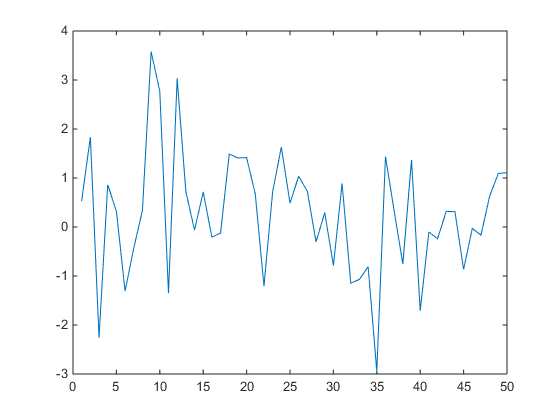
\includegraphics[width = 0.6\textwidth]{billeder/brownian}
\caption{Brownian Random Walk}
\label{fig:brownianrw}
\end{figure}
When looking at Brownian random walks it becomes apparent that the model might not reflect animal behaviour as it would be a bad strategy to visit the same area multiple times in a search. Only when you revisit a site with fast food regeneration would this strategy seem feasible.\\
Brownian motion obeys the rule of the central limit theorem. When the variance in equation \ref{eq:brownianm} gets sufficiently large the distribution will be very wide and the probability for $P(0)$ will be very low.

\subsection{Levy motion}
Lévy motion, also know as lévy flight or lévy walks, is a type of random walk where the step length generally follows a power law tailed distribution. In mathematically terms this can be shown as follows:
\begin{equation}
P($Step size$) \sim l ^{-\mu} ($for $ 0 < l $, $1 < \mu < 3$ and $ \mu = 1 + \alpha)
\label{eq:levyrw}
\end{equation}
In equation \ref{eq:levyrw} the $\alpha$ is the characteristic exponent. When the number of steps gets sufficiently large the distances converges to a stable distribution. Both distributions are fat tailed allowing large step sizes which would otherwise be classified as outliers in a Gaussian distribution. A two dimensional model of a levy flight can be seen in figure \ref{fig:levywalk1}.
\begin{figure}[H]
\centering
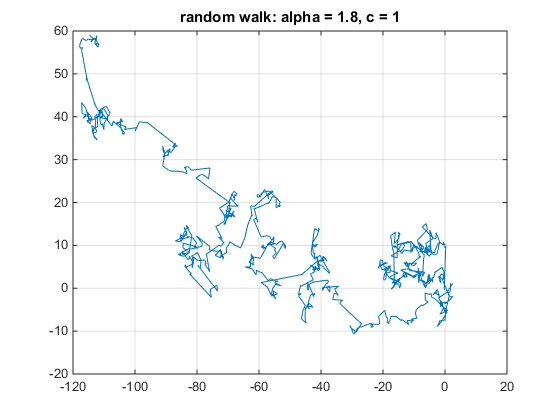
\includegraphics[width = 0.6\textwidth]{billeder/levywalk1}
\caption{Levy flight with 1000 steps and $\alpha = 1.8$}
\label{fig:levywalk1}
\end{figure}
Lévy walks have an addition limit in therms of step size. This is because of way acceleration works in levy flights. It is assumed that a flight takes zero or very little time. This is not true for walking. Walking has a finite velocity. In \cite{viswanathan2011the} the Lévy walk is described with a Dirac $\delta$-function to couple space and time. This can be seen in equation \ref{eq:levywalk} where $v$ is velocity and $\tau$ is the time it takes to move $l$.
\begin{equation}
P($Step size$) \sim l ^{-\mu}\delta (l - v\tau)
\label{eq:levywalk}
\end{equation}

\section{The Lévy alpha-stable distribution}
The skew Lévy $\alpha$-stable distribution is the most general case of stable distributions. The characteristic function is given by:
\begin{equation}
\varphi (t) = exp[itv - |ct|^{\alpha} (1-i\beta sign(t) tan[\frac{\alpha \pi}{2}])] $, for $ \alpha \neq 1
\end{equation}
and
\begin{equation}
\varphi (t) = exp[itv - |ct|^{\alpha} (1-i\beta sign(t) -(\frac{2}{\pi})ln|t|)] $, for $ \alpha = 1.
\end{equation}
where $i$ is the imaginary i, $v$ is the location parameter, $c$ is the scaling parameter, $\alpha$ is the characteristic exponent (or stability parameter) and $\beta$ is the skewness parameter. The ranges of these parameters are:\\
\begin{center}
$\alpha \in (0, 2]$\\
$\beta \in [-1, 1]$\\
$c \in (0, \infty)$\\
$v \in (-\infty, \infty)$\\
\end{center}
The characteristics for stable distribution entail when $\alpha = 2$ the distribution is reduced to a Gaussian distribution with variance $\sigma^2 = 2c^2$ and when $\alpha = 1$ and $\beta = 0$ the distribution is reduced to a Cauchy distribution. The variance is only defined when $\alpha = 2$. The mean is only defined when $1 < \alpha $ then the mean is equal to $v$.\\
The Probability Density function is found by Fourier transforming the characteristic function.\\
\begin{equation}
P(S) = \frac{1}{2\pi}\int_{-\infty}^{\infty} \varphi(t) exp[-itS] dt
\label{eq:fourier}
\end{equation}
The most simple version of the characteristic function is when $\beta = 0$ and $v = 1$. The characteristic function is reduced to:
\begin{equation}
\varphi (t) = exp[- |ct|^{\alpha}]
\label{eq:reducedcharfunc}
\end{equation}
It is then said that the distribution is a symmetric alpha-stable distribution or S$\alpha$S. The symmetry can be seen in figure \ref{fig:stablepdfsweep} where $\alpha$ is swept from 0.2 to 2. 
\begin{figure}[H]
\centering
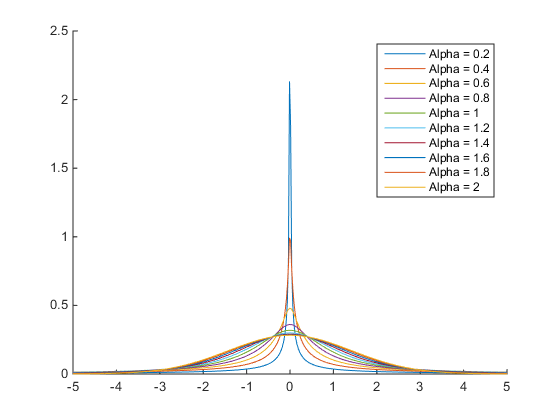
\includegraphics[width = 0.8\textwidth]{billeder/stblpdfsweep}
\caption{Stable distribution sweep of $\alpha$}
\label{fig:stablepdfsweep}
\end{figure}
The function seen in equation \ref{eq:reducedcharfunc} will be the basis of the simulation done in this study.


 

\section{Simulation}
This section contains the though process of the simulation part of this study. The simulations are performed in MATLAB.

\subsection{Implementing a data generator}
The simplest way of looking at a levy random walk is in two dimensions. When taking a step in a new direction two things are needed. A random angle in accordance to your old heading and a step size. An approximate generator of a levy flight is implemented using matlab code found on the stackexchange website\cite{firstlevy}. The generator can be seen in listing \ref{levyflightgen}.
\begin{lstlisting}[caption={Approximate levy flight generator},label=levyflightgen]
alpha=1.6;
s=1000;
for n=2:s;
    theta=rand*2*pi;
    f=rand^(-1/alpha);
    x(n)=x(n-1)+f*cos(theta);
    y(n)=y(n-1)+f*sin(theta);
end;
\end{lstlisting}
The step size follows a power law distribution but is limited by the rand which generates uniformly distributed random numbers. The model provides a basic model that is useful for understanding a levy flight generator.\\
Doing a further search for useful information on how to implement a generator led to the discovery of a series of matlab functions found on CSIRO Marine and Atmospheric research website\cite{betterlevy}. It becomes apparent that the levy flight generator found here makes use of stable random number generator\cite{stabrnd}. The generator can be seen in listing \ref{levyflightgen2}.  
\begin{lstlisting}[caption={Levy flight generator using a stable random number generator},label=levyflightgen2]
  r = stabrnd(alpha, beta, c, delta, 1, n);
  theta = 2*pi*rand(1, n);
  x(:, 1) = r.*cos(theta);
  x(:, 2) = r.*sin(theta);
\end{lstlisting}

\subsection{Implementing a parameter estimator}
Two parameter estimators have been implemented. A naive fitted distribution parameter estimator and a log|S$\alpha$S| parameter estimated based on a paper
\cite{XinyuMa1995}. The naive fitted distribution parameter estimator works by calculating the error term with respect to the histogram of the data. This is done for multiple instances of alpha. The best fitting alpha is output in the end. The distribution is made using a matlab toolbox\cite{stbltoolbox}.
\begin{algorithm}[H]
\caption{Naive fitted distribution parameter estimator algorithm}
\begin{algorithmic}
\For {$\alpha = 1$ to $1.8$ in steps of $0.1$}
\State $ Error(alpha) = (Distribution - Histogram)^2$
\EndFor
\State {$BestFit = FIND( MIN (  Error ( alpha ) )$}
\end{algorithmic}
\end{algorithm}
For the output of the Naive fitted distribution parameter estimator see the results chapter.\\

The log|S$\alpha$S| parameter estimator found in the paper by Xinyu Ma\cite{XinyuMa1995} uses the following equations derived in the paper:
\begin{equation}
\sigma^2 = \frac{\pi^2}{6}(\frac{1}{\alpha^2} + \frac{1}{2})
\end{equation}
\begin{equation}
\mu = C_e ( \frac{1}{\alpha} - 1) + \frac{1}{\alpha} log(\gamma)
\end{equation}
where $Y = log|X|$ and $C_e=0.57721566$(The Euler constant), $\alpha$ is characteristic exponent and $\gamma$ the scale. By utilising the new random variable Y based on our dataset X we can estimate $\alpha$ and $\gamma$ using mean and variance. Solving for  the parameters yields:
\begin{equation}
\hat{\alpha} = \sqrt{\frac{1}{\sigma^2 * \frac{6}{\pi^2} -\frac{1}{2}}}
\end{equation}
\begin{equation}
\hat{\gamma} = 10^{(\hat{\alpha} * ( \mu - C_e * ( \frac{1}{\hat{\alpha}} - 1) ) )}
\end{equation}
The estimated parameters are inserted into equation \ref{eq:reducedcharfunc}, with c = $\gamma$ and fourier transformed in accordance to equation \ref{eq:fourier}. The Probability density function is plotted against the histogram in the results section. The estimated parameters for multiple cases can also be found in the results section.
\chapter{Results}
Resultaternes plot med den naive metode.
Resultaternes plot med log|SaS| metode.

Tabel med Resultater for forskellige alpha.

\chapter{Gained Knowledge}

\chapter{Conclusion}
In this project a least squares solver has been implemented using High-Level Synthesis. Using the Vivado HLS tool, different directives has been applied and the effect analysed and used for comparison. With a starting point in the unoptimised implementation, it was possible to reduce the latency in the design at the expense of higher resource requirement. Likewise it was possible to reduce the resource requirement at the expense of higher latency. The Vivado HLS tool also uses iterative optimisation when synthesising the design to RTL.

The development in the project was made easier by the Vivado HLS tool. The tool provides an environment for faster development compared to designing and implementing using lower abstraction layers. The technology will still need to be adapted by researchers and developers as it not very mature yet.
%\include{filer/16References}


%%%% Kilder %%%%
\begingroup
	\raggedright
	\bibliography{bibtex/litteratur}							% Litteraturlisten inkluderes
\endgroup



\end{document}